\cotefile{43}
\scanpage{161}
% archive sheet number: 160
% L1
\uline{Cas des préschémas} loc. noeth.

% L2-5
Si $F$ est cohérent, les $\underline{\operatorname{Ext}}^i_Z(F,G)$ sont quasi-cohérents. On le voit par \unsure{exemple|récurrence} sur \unsure{la} suite spectrale de terme initial $\underline{H}^p_Z(\underline{\operatorname{Ext}}_{\mathcal O_X}(F,G))$, utilisant le fait qu'une extension de qu. coh. est \unsure{itou} \unsure{...}

% L6-8
On a un hom. canonique (\unsure{$Y$|$Z$} fermé)
\[
\left\{\begin{aligned}
1)\quad &\operatorname{Ext}^i_{\deleted{\unsure{Y}}}(X;F,G)\longleftarrow\varinjlim\operatorname{Ext}^i(X;F/{\unsure{\mathcal J|J}}^{n+1}F,G)\\
2)\quad &\underline{\operatorname{Ext}}^i_{\unsure{Y|\gamma}}(F,G)\longleftarrow\varinjlim\underline{\operatorname{Ext}}^i(F/\mathcal J^{\unsure{n+1}}F,G)
\end{aligned}\right.
\]

% L9-11
\uline{Th.} \inserted{Supposons $F$ \uline{cohérent}.} L'hom. 2) est un isom, \deleted{\unsure{$X$ loc. noeth.}}, et 1) est un isom si $X$ est noethérien.

% L12-14
On déduit \deleted{\unsure{de}} le \unsure{deuxième} isom du premier comme d'habitude, par la suite spectrale
\[
H^p(X,\underline{\operatorname{Ext}}^q_Y(F,G))\Longrightarrow\operatorname{Ext}_Y(X;F,G).
\]
% L15-18
L'énoncé est de nature \uline{\unsure{loc.|locale}}, on peut supposer $X$ affine. Pour $i=0$, c'est évident, il reste à \deleted{\unsure{examiner}} prouver que si $G$ provient d'un module \uline{injectif}, on a $\underline{\operatorname{Ext}}^i_Y(F,G)=0$ pour $i>0$.

% L19
Or on regarde $\operatorname{Ext}^p_A(\unsure{M|N},\underline{H}^q_J(N))$ et on voit que si $N$

\scanpage{162}
% archive sheet number: 161
% L1-2, in the orientation of the scan
injectif, alors les $H^q_J(N)$ sont nuls pour $q>0$, et $H^0_J(N)$ est injectif, OK \unsure{----}

% The remaining writing is sideways on the scan; transcribed in its reading direction.
% T1: upper cancelled table
\deleted{Ind pro}
\[
\underline{\operatorname{Ext}}^{\unsure{i|1}}(F,G)
\]
\diagram{$\deleted{\begin{array}{c|c|c|c|c|c|c|c|c|c}
\underline{\operatorname{Hom}}(F,G)&\mathbb Z/\unsure{\ell|l}\mathbb Z&\unsure{\mathbb Z/p\mathbb Z}&{\unsure{\mu|H}}_p&\alpha_p&{\unsure{\mathbb G|G}}_m&\mathbb G_a&\unsure{\mathbb V|V}&\unsure{\mathbb Z|A}&A\\\hline
\mathbb Z/\ell\mathbb Z&\mathbb Z/\ell\mathbb Z&&0&0&\mu_\ell&0&0&0&{}_{\ell}A\\\hline
\mu_p&0&&\mathbb Z/p\mathbb Z&&&&&&
\end{array}}$}

% T2: heading and abandoned heading
Tableau des \uline{Hom}

\deleted{$\mu_p\quad\alpha_p\quad\mathbb Z/p\mathbb Z\quad\mathbb Z/\ell\mathbb Z$ Tableau des $\underline{\operatorname{Ext}}$}

% D1: small matrix, above the right corner of the main table
\diagram{$\left(\begin{array}{ccc}
\mathbb Z/p\mathbb Z&0&0\\
\alpha_p&\mathbb G_a&0\\
\mu_p&\alpha_p&\mathbb Z/p\mathbb Z
\end{array}\right)$}

% T3: main table. Blank cells in T1 are blank in the manuscript.
\diagram{$\begin{array}{c|c|c|c|c|c|c|c|c|c}
&\mathbb Z/\ell\mathbb Z&\mathbb Z/p\mathbb Z&\alpha_p&\mu_p&\mathbb G_m&\mathbb G_a&\mathbb Z&\mathbb V&A\\\hline
\mathbb Z/\ell\mathbb Z&\mathbb Z/\ell\mathbb Z&0&0&0&\mu_\ell&0&0&0&{}_{\ell}A\\\hline
\mathbb Z/p\mathbb Z&0&\mathbb Z/p\mathbb Z&\alpha_p&\mu_p&\mu_p&\mathbb G_a&0&\mathbb V&{}_{p}A\\\hline
\alpha_p&0&0&\mathbb G_a&\alpha_p&\alpha_p&\mathbb G_a&0&\text{\tikz[baseline=(c.base)]{\node[draw,rounded corners=6pt,inner sep=2pt] (c) {$\unsure{\text{gros}|\text{quoi}}?$};}}&\deleted{\unsure{\mathbb V}({\unsure{t}}_A^{\unsure{1-p|1/p}})}\ {?}\\\hline
\mu_p&0&0&0&\mathbb Z/p\mathbb Z&\mathbb Z/p\mathbb Z&0&0&0\deleted{\unsure{?}}&\deleted{({\unsure{t}}_A^{p})_{\unsure{k}}}\ {?}\\\hline
\mathbb G_m&0&0&0&0&\mathbb Z&0&0&0&0\\\hline
\mathbb G_a&0&0&\text{\tikz[baseline=(c.base)]{\node[draw,rounded corners=6pt,inner sep=2pt] (c) {$\unsure{\text{gros}|\text{quoi}}$};}}&\mathbb V&\mathbb V&\boxed{\begin{gathered}\deleted{\unsure{\mathbb G_a}}\\{\unsure{\text{Imm}}}^{\unsure{2}}\end{gathered}}&0&\text{\tikz[baseline=(c.base)]{\node[draw,rounded corners=6pt,inner sep=2pt] (c) {$\mathbb G_a?$};}}&\unsure{\text{gros}}\\\hline
\mathbb Z&\mathbb Z/\ell\mathbb Z&\mathbb Z/p\mathbb Z&\alpha_p&\mu_p&\mathbb G_m&\mathbb G_a&\mathbb Z&\mathbb V&A\\\hline
\mathbb V&0&0&\mathbb G_a&\deleted{\unsure{\mathbb G}}\mathbb G_a&\mathbb G_a&\text{\tikz[baseline=(c.base)]{\node[draw,rounded corners=6pt,inner sep=2pt] (c) {$\mathbb G_a$};}}\unsure{!}&0&\text{\tikz[baseline=(c.base)]{\node[draw,rounded corners=6pt,inner sep=2pt] (c) {$\unsure{\text{Imm}}$};}}&\underline{V}(\omega_A)\\\hline
A&0&0&0&0&0&0&0&0?&\mathbb Z^{\unsure{n|m}}
\end{array}$}
% margin note written sideways
\margin{\unsure{con|conn}\ $\left\{\begin{array}{c}\alpha_p\\\mu_p\\\mathbb G_m\\\mathbb G_a\end{array}\right.$}
% margin note written sideways
\margin{$\underline{\operatorname{Hom}}(\alpha_p,\mathbb G_m)$}
% margin note written sideways
\margin{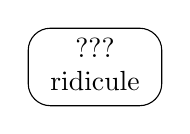
\begin{tikzpicture}\node[draw,rounded corners=8pt,inner sep=2pt] {\begin{tabular}{c}???\\\unsure{ridicule}\end{tabular}};\end{tikzpicture}}

\scanpage{163}
% archive sheet number: 162
% L1-2
\[
\underline{\operatorname{Hom}}(G,H)=0\quad\text{si}\quad
\left\{\begin{array}{l}G\text{ à fibres géom connexes}\\H\text{ non ramifié sur }S\end{array}\right.
\]
% L3
\[
\underline{\operatorname{Hom}}(\mathbb Z/n\mathbb Z,G)\simeq {}_nG\qquad\text{d'où lignes 1,2}
\]
% L4
\[
\underline{\operatorname{Hom}}(\mathbb Z,G)\simeq G\qquad\text{d'où ligne 7}
\]
% L5-8
\diagram{\begin{tikzcd}[ampersand replacement=\&,column sep=small,row sep=small]
\underline{\operatorname{Hom}}(\alpha_p,G)\arrow[d,phantom,"\simeq"{rotate=90}]\&\simeq\operatorname{Ker}\bigl(\underline V(\omega_G)\xrightarrow{\text{puiss. }p.\text{ième}}\underline V(\omega_G)\bigr)\\
\underline{\operatorname{Hom}}(\alpha_p,\underline{\unsure{\mathscr U|\mathcal U}}_G^{(1)})\&\begin{gathered}\underline{\unsure{t|\mathfrak t}}_G\\\text{schéma de Lie de }G\end{gathered}
\end{tikzcd}}
\margin{d'où ligne 3 moins l'avant-dernière ----}
% L9
\[
\underline{\operatorname{Hom}}({\unsure{\mu|H}}_p,G)\simeq\operatorname{Ker}\bigl(\underline V\omega_G)\xrightarrow{\text{id-puiss. }p\text{ième}}\underline V\omega_G)\bigr)\qquad\text{d'où ligne 4}
\]
% L10-11
$\underline{\operatorname{Hom}}({\unsure{\mathbb G|G}}_m,G)$ est un foncteur ``non ramifié'' d'où ligne 5

% L12-13
$\underline{\operatorname{Hom}}(A,G)$ est un foncteur ``non ramifié'' d'où (partiellement) ligne 6.

% L14
\[
\underline{\operatorname{Hom}}(\unsure{\mathbb V|V},G)\simeq\underline V(\omega_G)\qquad\text{d'où ligne 8}
\]

% L15-18
Cas difficiles
\diagram{$\begin{array}{l|l}
a)\quad\underline{\operatorname{Hom}}(\mathbb G_a,G)&b)\quad\underline{\operatorname{Hom}}(G,\mathbb V)\\
G=\alpha_p,\mathbb G_a,\mathbb V,\ //A&G=\alpha_p,\mathbb G_a,\mathbb V_{\unsure{k|a}},\ //A
\end{array}$}
(implique b) pour $G=\mathbb G_a,\mathbb V,\alpha_p$)

% L19-20
Il y a essentiellement \deleted{deux}\inserted{quatre} types ``délicats'' ------

\scanpage{164}
% archive sheet number: 163
% T1, landscape table, read by rows
\diagram{\begin{tikzpicture}
\node[inner sep=0] (t) {$\begin{array}{c|c|c|c|c|c|c|c|c}
&{\unsure{\mu|H}}_p&W_{11}&\mathbb Z/\unsure{\ell|l}\mathbb Z&\mathbb Z/p\mathbb Z&{\unsure{\mathbb G|G}}_m&\mathbb G_a&\mathrm{Ab}&\mathbb Z\\\hline
{}_p\mathbb G_m=\mu_p&\begin{gathered}\inserted{\text{par dualité}}\\\mathbb Z/p\end{gathered}&0&0* &*0&\deleted{\unsure{\mathbb Z/p}}0&0&\operatorname{Ext}(\mathbb G_m,{}_pA)&0*\\\hline
{}_F\mathbb G_a={\unsure{\mathbb W|W}}_{11}-&0&\mathbb G_a^2\ \text{\tikz[baseline=-.5ex]\node[draw,circle,inner sep=2pt]{?};}&0*&*0&0&\text{\tikz[baseline=-.5ex]\node[draw,circle,inner sep=2pt]{?};}&\operatorname{Ext}(\mathbb G_a,{}_pA)&0*\\\hline
\mathbb Z/\ell\mathbb Z&0*&0*&\mathbb Z/\ell\mathbb Z&0&\phi\ 0&\phi\ 0&\phi\ 0&\phi\ \mathbb Z/\ell\\\hline
\mathbb Z/p\mathbb Z&0*&0*&0&\mathbb Z/p\mathbb Z&\phi\ 0&\mathbb G_a&\phi\ 0&\phi\ \mathbb Z/p\mathbb Z\\\hline
\mathbb G_m&\mathbb Z/p\mathbb Z&0&\begin{gathered}\operatorname{Hom}(T(\mathbb G_m),\mathbb Z/\ell\mathbb Z)\\\simeq\mathbb Z/\ell\mathbb Z\end{gathered}&0\ \unsure{0|\circ}&0&0&\varinjlim\operatorname{Ext}(\mathbb G_m,{}_nA)&\\\hline
\mathbb G_a&0&\text{\tikz[baseline=-.5ex]\node[draw,circle,inner sep=2pt]{?};}&0\ \unsure{0|\circ}&\text{\tikz[baseline=-.5ex]\node[draw,circle,inner sep=2pt]{?};}&0&\text{\tikz[baseline=-.5ex]\node[draw,circle,inner sep=2pt]{?};}&\varinjlim\operatorname{Ext}^1(\mathbb G_a,{}_nA)&\smash{\text{\Huge ?}}\\\hline
\mathrm{Ab}&\multicolumn{4}{c|}{\operatorname{Hom}(T(A),G),\quad\unsure{h}}&(\mathrm{Ab})'&H^1(\mathrm{Ab},\underline{\unsure{\mathcal O|O}})&\deleted{\unsure{finis}}\ \text{----}&\\\hline
\mathbb Z&0*&0*&0*&0*&0*&0*&0*&0*
\end{array}$};
\draw ([xshift=-3pt,yshift=-20pt]t.north west) -- ++(-4pt,0) |- ([xshift=-3pt]t.west);
\draw ([xshift=-3pt,yshift=-3pt]t.west) -- ++(-4pt,0) |- ([xshift=-3pt]t.south west);
\end{tikzpicture}}

% L1-2, below table, left
$\phi\quad\operatorname{Ext}^1(\mathbb Z/n\mathbb Z,G)={}^nG$

\deleted{\unsure{donc}} $\operatorname{Ext}^1(F,G)=0$ si $F$ discret fini; $G$ divisible

% L3-7, below table, left
$*\quad$\unsure{deux groupes} \deleted{\unsure{finis}}, l'un \deleted{\unsure{étale}}\inserted{discret}, l'autre \unsure{radiciel|unipotent}, ont des ext. mutuelles nulles

% L8, outlined central heading
\figure{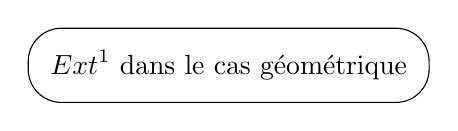
\begin{tikzpicture}\node[draw,rounded corners=12pt,inner sep=8pt] {$\operatorname{Ext}^1$ dans le cas \uline{géométrique}};\end{tikzpicture}}

% L9-10, heavily cancelled lower block
\deleted{N.B. $\operatorname{Ext}^2(\unsure{\mathbb G_a|\mathbb G_m},\mathbb G_m)\ne0$ \unsure{cf.} \illegible{4}}

% L11-12
\tikz[baseline=-.5ex]\node[draw,circle,inner sep=4pt]{?};\quad\uline{Consulter travaux Serre}

pour déterminations explicites

% Right-hand marginal note
\margin{Il n'est pas \unsure{clair} qu'il y ait lieu de considérer des ext. de $\mathbb G_a$, $\mathbb G_m$ ou $\mathrm{Ab}$ par $\mathbb Z$; on trouve \unsure{dans tous des} $0$}

\scanpage{165}
% archive sheet number: 164
% T1
\diagram{$\begin{array}{c|c|c|c|c|c|c}
&{\unsure{\Gamma|\mathcal T}}'&U&{\unsure{\mathbb G|G}}_m&\mathbb G_a&\mathrm{Ab}\ \text{simple}&\mathbb Z\\\hline
\begin{gathered}\unsure{a')}\quad\Gamma\left\{\begin{array}{l}\mathbb Z/\unsure{\ell|l}\mathbb Z\\\mathbb Z/p\mathbb Z\end{array}\right.\quad\unsure{b')}\end{gathered}&\begin{gathered}\text{groupe fini ordinaire}\\\unsure{\simeq}\operatorname{Hom}(\Gamma,\Gamma')\end{gathered}&\begin{gathered}0\text{ ou}\\\unsure{\text{tt}|\simeq}\text{ groupe radiciel simple}\end{gathered}&\begin{gathered}\text{groupe }\unsure{\text{simple}|\text{infini}}\\(\unsure{\text{exp.}|\text{ét.}}\text{ ou radiciel})\end{gathered}&\begin{gathered}0\\\text{ou }\mathbb G_a\end{gathered}&\begin{gathered}\text{groupe fini}\\\unsure{\text{sép.}|\text{exp.}}\ \text{ou mixte}\end{gathered}&0\\\hline
\begin{gathered}a)\quad U\left\{\begin{array}{l}{}_p\mathbb G_m=D(\mathbb Z/p\mathbb Z)\\{}_F\mathbb G_a\end{array}\right.\quad b)\end{gathered}&0&\begin{array}{c|c}\mathbb Z/p\mathbb Z&\deleted{\unsure{0}}\text{\tikz[baseline=-.5ex]\node[draw,circle,inner sep=1pt]{$0$};}\\\hline{}_F\mathbb G_a&\mathbb G_a\end{array}&\begin{gathered}\mathbb Z/p\mathbb Z\\{}_F\mathbb G_a\end{gathered}&\begin{gathered}0\\\mathbb G_a\end{gathered}&\begin{gathered}\text{groupe }(\mathbb Z/p\mathbb Z)^n\\{}_F\mathbb G_a^m\times\mathbb G_a^n\end{gathered}&0\\\hline
c)\quad\mathbb G_m&0&\times\,0&\mathbb Z&0&0&0\\\hline
\unsure{f')}\quad\mathbb G_a&0&\begin{array}{c|c}\subset\unsure{\mathbb W_{\infty,1}|W_{\infty,1}|W_{\infty}}\,\times{}^{(\alpha)}&{}^{(\beta)}\\\text{(Hom anneaux}&\unsure{\simeq\mathbb V^n|\simeq\mathbb V^\infty}\\\unsure{\text{non comm.}}&\text{quotient}\\\unsure{\text{polynômes}}\text{)}&\text{de }\unsure{\leftarrow\mathbb V^n|\simeq\mathbb V^n}\end{array}&\begin{gathered}\text{radiciel }\deleted{\unsure{\text{inf}}}\\=\operatorname{Hom}(\mathbb G_a,{}_p\mathbb G_m)\end{gathered}&\unsure{\mathbb V|V}\ \times&\begin{gathered}\text{radiciel}\\=\operatorname{Hom}(\mathbb G_a,U)\end{gathered}&0\\\hline
 d)\quad\mathrm{Ab}\ \text{simple}&0&\times\,0&0&0&\begin{gathered}\text{groupe discret}\ \unsure{\text{sans torsion}}\\\text{ord. de type fini}\end{gathered}&0\\\hline
\unsure{e)}\quad\mathbb Z\ \text{groupe ordinaire}&\Gamma&U&\mathbb G_m&\mathbb G_a&\mathrm{Ab}\ \text{simple}&\mathbb Z
\end{array}$}

% L1
\figure{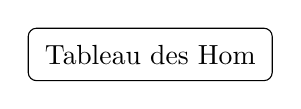
\begin{tikzpicture}\node[draw,rounded corners=3pt,inner sep=6pt] {Tableau des \uline{Hom}};\end{tikzpicture}}
% L2-4
\[
\begin{aligned}
\underline{\operatorname{Hom}}(\text{grp connexe},\text{grp discret ordinaire})&=0\\
\underline{\operatorname{Hom}}(\mathbb G_m,\text{grp ne }\unsure{\text{contenant}}\text{ pas }\unsure{\simeq|\text{de}}\ \mathbb G_m)\unsure{\dagger}&=0\\
\underline{\operatorname{Hom}}(\mathrm{Ab},\text{grp linéaire})&=0
\end{aligned}
\]
% L5
${\unsure{\mathscr S|\mathbb S|S}}_\infty\longrightarrow\mathbb G_a$ hom d'anneaux de $\mathscr S_\infty$ dans $\mathbb G_a$

% L6
\deleted{\unsure{(Hom) (Hom)}}

% L7-8
\[
\operatorname{Hom}(\mathbb G_a,{}_p\mathbb G_m)
\]
\[
\unsure{k\{[t]\}|k[[t]]}\longleftarrow k[t]/(1-t)^p
\]
% L9-10
élément nilpotent en $k\{[t]\}$, néc. de la forme $\sum a_i t^i$, les $a_i^p=0$

% L11-12
\[
\deleted{\Delta(\sum a_i t^i)=}\qquad 1+a_1t+a_2t^2\ \unsure{\cdots}\ +a_nt^n\qquad a_i^{\unsure{\nu|v|p}}=0
\]
\[
P(t+t')=P(t)P(t')
\]

% margin note, lower right
\margin{$\alpha)$ C'est le \deleted{grp}\inserted{groupe (pro-algébrique)} $D(\mathbb G_a)$ de Cartier ---- C'est un grp \uline{radiciel infini}}
\margin{$\beta)$ C'est un grp \unsure{$k$-simple} infini sur $k$.}

\scanpage{167}
% archive sheet number: 166
% L1-5
\uline{Lemme} Soient $G,\unsure{\gamma|\sigma}$ deux schémas en groupes \inserted{comm} sur $S$, tels que $\unsure{/^{\circ}}\ \deleted{\underline{\underline{\operatorname{Hom}}}_{S,\unsure{\text{pointés}}}(G,\gamma)=0}\inserted{\underline{\underline{\operatorname{Hom}}}}$ [par exemple $G$ à fibres géométriquement connexes, et $\gamma$ non ramifié sur $S$], $\gamma$ fid plat sur $S$ pour simplifier. Alors

% L6, with annotation below codomain
\[
\operatorname{Ext}_{S\text{-gr}}(G,\gamma)\longrightarrow\underbrace{H^1(G,\gamma_G)}_{\substack{\text{classes de fibrés}\\\text{principaux homogènes}}}\tag*{(*)}
\]
% L7-10
est \uline{injectif}, et $/^{\circ}$ a pour image \unsure{les ensemble|l'ensemble} des éléments \uline{primitifs} de $H^1(G,\gamma_G)$ [i.e. ceux dont l'image dans $H^1(S,\gamma)$ sont nulles, et satisfaisant $\pi^{\unsure{*|\alpha}}(\unsure{\xi|\zeta})-\operatorname{pr}_1^*(\xi)-\operatorname{pr}_2^*(\xi)=0$]

% margin note written sideways
\margin{$/^{\circ}$ Tout hom $G\times_S G\longrightarrow\gamma$ qui est nul sur $e\times_S G$ et sur $G\times_S e$ est nul}
% margin note written sideways
\margin{$/^{\circ}$ Si \unsure{tt S-morph.} $(G/\unsure{k|S})^n\longrightarrow\gamma$ provient d'un hom $S\longrightarrow\gamma$ (pour $n=1,2,3$) alors \deleted{\unsure{dans ce cas}}}

% L11-12
\uline{Dém} Soit
\[
0\longrightarrow\gamma\overset{\alpha}{\unsure{-|\longrightarrow}}E\overset{\beta}{\unsure{-|\longrightarrow}}G-0
\]
% L13-20
une extension de $S$-groupes [$E\unsure{-|\longrightarrow}G$ fid plat], supposons qu'elle définisse $E$ comme un fibré principal \uline{trivial} sur $G$, i.e. qu'il existe une section $\unsure{\varphi|\phi}:G\longrightarrow E$. Soit $e_G:S\longrightarrow G$ la section unité, d'où une section $\varphi e_G\unsure{\leftarrow|=}\varphi(e_G)$ de $E$ sur $S$, \unsure{dont|et} l'image par $\beta$ est la section unité $e_G$, donc qui est de la forme $\alpha(u)$, $u\in\gamma(S)$, corrigeant

\scanpage{168}
% archive sheet number: 167
% L1-6
$\unsure{\varphi|\phi}$ par $u$, on peut supposer que $\varphi$ transforme section unité en section unité. Prouvons que $\varphi$ est \uline{\unsure{multiplicative|multiplicatif}}. En effet, $\pi'(\varphi\times_S\varphi)-\varphi\circ\pi$ est un $S$-morphisme $G\times G\longrightarrow\unsure{\gamma|\sigma}$, qui est nul sur $G\times_S e$ et $e\times_S G$.
\diagram{\begin{tikzcd}[ampersand replacement=\&]
G\times G\arrow[r,no head,"\varphi\times\varphi"]\arrow[d,no head,"\pi"']\&E\times E\arrow[d,"\pi'"]\\
G\arrow[r,"\varphi"']\&E
\end{tikzcd}}
% L7
Donc cela prouve l'injectivité ----.

% L8-12
Le fait que l'image de $\operatorname{Ext}_{S\text{-gr}}(G,\gamma)\unsure{-|\longrightarrow}H^1(G,\gamma)$ ait les propriétés indiquées, est \deleted{\unsure{pure.}} vrai sans hyp. sur $G,\gamma$, compte tenu de la construction des fibrés associés.
\diagram{\begin{tikzcd}[ampersand replacement=\&]
\gamma\times\gamma\&E\times E\arrow[r]\arrow[d]\&G\times G\arrow[d]\\
\gamma\&E\arrow[r]\&G
\end{tikzcd}}

% L13-16
Pour la réciproque, \inserted{Sous les conditions dites}, on voit que \deleted{\unsure{le fait}}\inserted{si} $E$ est fibré pr. homog sur $G$ \deleted{\unsure{soit}} de classe primitive, il existe \deleted{donc} une section $e_E$ de $E/S$ au dessus de celle de $G/S$.

% slanted
\margin{Précision: étant donné une section $e_E$ de $E$ sur $e_G$, $\exists$ une structure de $S$-groupe unique sur $E$ ayant $e_E$ comme section unité, et telle que $\unsure{E|G}$ \unsure{soit un} $\gamma$-\unsure{groupe}, $E\longrightarrow G$ \unsure{un morphisme} \illegible{2}.}

% L17-19
De plus, il existe un morphisme $E\times E\unsure{-|\longrightarrow}E$ compatible avec $\gamma\times\gamma\longrightarrow\gamma$ et rendant comm. le diagramme
\diagram{\begin{tikzcd}[ampersand replacement=\&]
E\times E\arrow[r]\arrow[d,no head]\&G\times G\arrow[d,no head]\\
E\arrow[r,no head]\&G
\end{tikzcd}}
% L20-22
Il y a unicité à translation près dans $E$ par un élément de \deleted{$\unsure{\gamma}$}\inserted{$\operatorname{Hom}(G\times_S G,\gamma)\simeq\operatorname{Hom}(S,\gamma)$} et dont on peut profiter pour \unsure{condition|modifier} \deleted{(de façon unique)} à transformer $(e_E,e_E)$ en $e_E$.

\scanpage{169}
% archive sheet number: 168
Je dis que cette loi de composition fait de $E$ un \uline{schéma en groupes}. Il faut vérifier

(i) L'associativité, qui s'exprime par l'égalité de \uline{deux morphismes} $E\times E\times E\unsure{-|\longrightarrow}E$ au dessus de $G\times G\times G-G$, compatibles avec $\unsure{\gamma|\sigma}\times\gamma\times\gamma\longrightarrow\gamma$ ; cela résulte du fait qu'il y a \uline{un seul} tel morphisme, à translation près par un élément de $\operatorname{Hom}_S(G\times G\times G,\gamma)\simeq\gamma(S)$, donc un seul pour lequel l'unité entre en l'unité.

(ii) $e$ est l'unité, $\unsure{\bar m|\simeq}$ argument, \deleted{\unsure{pour}} \unsure{prouver} que deux hom $E-E$ sont l'identité.

(iii) Existence d'une symétrie de $E$

Voir l'exposé du livre de Serre, page 183.

\noindent ----

\noindent\rule{.72\linewidth}{.3pt}

Application au cas où $\gamma$ sur $\deleted{E}S$ est \uline{étale}, \inserted{et $G$ à fibres géom. conn.}

\uline{Alors}
\[
\operatorname{Ext}^{\unsure{1|{}}}_{S\text{-gr}}(G,\gamma)\unsure{\simeq|\cong}\operatorname{Ext}^{1}_{S_0\text{-gr}}(G_0,\gamma_0)
\]
où $S_0=S_{\mathrm{réd}}$, $G_0=G\times_S S_0$, $\gamma_0=\unsure{G|\gamma}\times_S S_0$. Ceci \unsure{est|vaut} plus gén. si $S_0\longrightarrow S$ est un homéom. universel quelconque. \deleted{Ceci permet l'application}

% slanted
\margin{N.B. Ce résultat est valable de façon indépendante de la prop. plus haut, si on suppose $G$ à fibres connexes --------}

\scanpage{170}
% archive sheet number: 169
\deleted{à \unsure{des cas} \illegible{1} \unsure{méthodes} \unsure{de descente} \unsure{fid.}}

D'ailleurs \deleted{\unsure{et}} comme une extension de $G$ par $\unsure{\gamma|\sigma}$ \unsure{n'a pas d'autom. non trivial}, on peut appliquer à $\operatorname{Ext}_{S\text{-gr}}(G,\gamma)$ les méthodes de descente [ainsi, pour $S'$ variable \inserted{\unsure{réd.}}, on obtient un foncteur en $S'$ compatible avec la descente fid. plate ....].

\unsure{Prenons}, p.ex. $G={\unsure{\mathbb G|G}}_a$, $\gamma=\mathbb{Z}/p\mathbb{Z}$, on trouve (\unsure{sous réserve|sans recours} \unsure{tt|et} \unsure{en|un} plus d'hypothèses noethériennes)
\[
\operatorname{Ext}_{S\text{-gr}}(\mathbb{G}_a,\mathbb{Z}/p\mathbb{Z})\simeq\Gamma(S,{\unsure{\mathscr O|\mathcal O|O}}_S^{p^{-\infty}}).
\]
% slanted
\margin{Pour la dém, cf exposé Groth. au séminaire \unsure{Chevalley|Chev.} sur les groupes algébriques I (Exposé 7)}
\[
\mathscr{O}_S^{p^{-\infty}}=\varinjlim_n(\mathscr{O}_S,n),
\]
avec l'hom $(\mathscr{O}_S,n)\longrightarrow(\mathscr{O}_S,m)$ défini par $x\longmapsto x^{p^{m-n}}$. On peut donc dire que le foncteur $\underline{\underline{\operatorname{Ext}}}_{S\text{-gr}}(\unsure{\mathbb{G}_S|\mathscr{O}_S},\mathbb{Z}/p\mathbb{Z})$ est représentable \deleted{par le} \inserted{dans la catégorie des} préschémas $p$-parfaits sur $S$.....

\scanpage{171}
% archive sheet number: 170
Dualité de Cartier des groupes \unsure{alg|alg.} affines et groupes formels

\scanpage{172}
% archive sheet number: 171
\diagram{$\begin{array}{c|c|c|c}
\begin{smallmatrix} &F\\ V&\diagdown\end{smallmatrix}&\text{isom}&\text{épim}&\text{nilpotent}\\ \hline
\text{isom}&\text{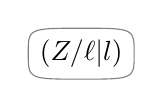
\begin{tikzpicture}[baseline=(q.base)]\node[inner sep=4pt] (q) {$(\mathbb Z/\unsure{\ell|l})$};\draw[gray,thin] (q.north) .. controls (q.north east) and (q.north east) .. (q.east) .. controls (q.south east) and (q.south east) .. (q.south) .. controls (q.south west) and (q.south west) .. (q.west) .. controls (q.north west) and (q.north west) .. cycle;\end{tikzpicture}}&\text{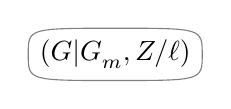
\begin{tikzpicture}[baseline=(q.base)]\node[inner sep=4pt] (q) {$({\unsure{\mathbb G|G}}_m,\mathbb Z/\ell)$};\draw[gray,thin] (q.north) .. controls (q.north east) and (q.north east) .. (q.east) .. controls (q.south east) and (q.south east) .. (q.south) .. controls (q.south west) and (q.south west) .. (q.west) .. controls (q.north west) and (q.north west) .. cycle;\end{tikzpicture}}&\text{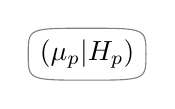
\begin{tikzpicture}[baseline=(q.base)]\node[inner sep=4pt] (q) {$(\unsure{\mu_p|H_p})$};\draw[gray,thin] (q.north) .. controls (q.north east) and (q.north east) .. (q.east) .. controls (q.south east) and (q.south east) .. (q.south) .. controls (q.south west) and (q.south west) .. (q.west) .. controls (q.north west) and (q.north west) .. cycle;\end{tikzpicture}}\\[1.2em]\hline
\begin{gathered}\deleted{\text{épim}}\\\text{mono}\end{gathered}&\begin{gathered}\text{discret \unsure{sép|si|ss}}\\ \text{\unsure{sans} }\unsure{V|p}\text{-torsion}\\(\mathbb Z/\ell,\mathbb Z)\deleted{\unsure{\mathbb Q}}\end{gathered}&\begin{gathered}\text{\unsure{multiplicatif} }\unsure{\times|+}\text{\unsure{simple|lisse}}\\\deleted{\text{\unsure{chaque groupe}}}\\\deleted{\text{\unsure{discret} }\unsure{p}\text{\unsure{-tors.}}}\\(\mathbb G_m,\mathbb Z/\ell\mathbb Z,\mathbb Z)\end{gathered}&\text{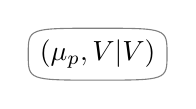
\begin{tikzpicture}[baseline=(q.base)]\node[inner sep=4pt] (q) {$(\mu_p,\unsure{\mathbb V|V})$};\draw[gray,thin] (q.north) .. controls (q.north east) and (q.north east) .. (q.east) .. controls (q.south east) and (q.south east) .. (q.south) .. controls (q.south west) and (q.south west) .. (q.west) .. controls (q.north west) and (q.north west) .. cycle;\end{tikzpicture}}\\[1.2em]\hline
\text{nilpotent}&\text{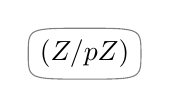
\begin{tikzpicture}[baseline=(q.base)]\node[inner sep=4pt] (q) {$(\mathbb Z/p\mathbb Z)$};\draw[gray,thin] (q.north) .. controls (q.north east) and (q.north east) .. (q.east) .. controls (q.south east) and (q.south east) .. (q.south) .. controls (q.south west) and (q.south west) .. (q.west) .. controls (q.north west) and (q.north west) .. cycle;\end{tikzpicture}}&\text{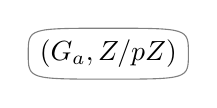
\begin{tikzpicture}[baseline=(q.base)]\node[inner sep=4pt] (q) {$(\mathbb G_a,\mathbb Z/p\mathbb Z)$};\draw[gray,thin] (q.north) .. controls (q.north east) and (q.north east) .. (q.east) .. controls (q.south east) and (q.south east) .. (q.south) .. controls (q.south west) and (q.south west) .. (q.west) .. controls (q.north west) and (q.north west) .. cycle;\end{tikzpicture}}&\begin{gathered}\deleted{\text{\unsure{groupe fini radiciel}}}\\\text{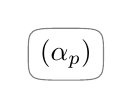
\begin{tikzpicture}[baseline=(q.base)]\node[inner sep=4pt] (q) {$(\alpha_p)$};\draw[gray,thin] (q.north) .. controls (q.north east) and (q.north east) .. (q.east) .. controls (q.south east) and (q.south east) .. (q.south) .. controls (q.south west) and (q.south west) .. (q.west) .. controls (q.north west) and (q.north west) .. cycle;\end{tikzpicture}}\end{gathered}\\\hline
\end{array}$}

Propriétés de $F,V$, \unsure{caractérisant} \unsure{l'Existence|l'existence|l'éclatement} de séries de composition ayant des propriétés données ----

\figure{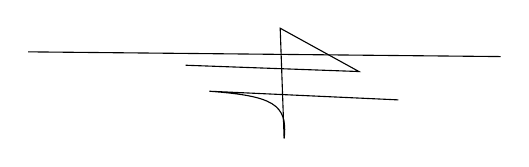
\begin{tikzpicture}[x=1cm,y=1cm]
\draw (0,0)--(6,-.06);
\draw (2,-.17)--(4.2,-.25)--(3.2,.30)--(3.25,-1.1);
\draw (4.7,-.61)--(2.3,-.50) .. controls (3.1,-.56) and (3.3,-.66) .. (3.25,-1.1);
\end{tikzpicture}}

% paper watermark: VELIN EXTRA (not author text)

\scanpage{173}
% archive sheet number: 172
\diagram{$\begin{array}{ccccccccc|c}
{\unsure{\mathbb G|G}}_m&\mathbb Z/\unsure{\ell|l}\mathbb Z&\unsure{\mu_p|H_p}&(\mathbb G_a&\alpha_p&\unsure{\mathbb V|V})&\mathbb Z/p\mathbb Z&\mathbb Z/\ell\mathbb Z&\mathbb Z&\mathrm{Ab}\\
F\text{ épim}&\left.\begin{matrix}F\\V\end{matrix}\right\}\text{isom}&F=0&F\text{ épim}&F=0&F=0&F\text{ isom}&\left.\begin{matrix}F\\V\end{matrix}\right\}\text{isom}&F\text{ isom}&F\text{ épim}\\
V\text{ isom}&&V\text{ isom}&V=0&V=0&V\text{ \unsure{monom|épimom}}&V=0&&V\text{ monom}&V\text{ n'importe quoi}\\
&&\multicolumn{4}{c}{\text{\begin{tikzpicture}\draw (0,.16)--(0,0)--(4.7,0)--(4.7,.16);\draw (3.1,0)--(3.1,.16);\end{tikzpicture}}} & * &&&
\end{array}$}

\[
\begin{aligned}
F\text{ isom}&:\quad\text{groupe discret séparable}\\
F^n=0&:\quad\text{groupe infinitésimal}
\end{aligned}
\]
\[
F\text{ épim}\quad :\quad \text{groupe \inserted{ind-}\uline{algébrique} séparable}
\]
$\underset{?}{\Longrightarrow}$ (peut avoir un quotient $\mathbb Z$, mais pas de facteur de composition $\mathbb V$)

i.e. pas de partie infinitésimale

\[
\begin{aligned}
V\text{ isom}&:\quad\text{groupe multiplicatif}\\
V^n=0&:\quad\text{groupe \inserted{algébrique} unipotent}
\end{aligned}
\]
\[
V\text{ \deleted{\unsure{épim}}\unsure{monom|épimom}}\quad :\quad\deleted{\text{\unsure{groupe inf.}}}\quad\text{\inserted{algébrique}}
\]
$\overset{?}{\Longrightarrow}$ pas de partie unipotente en facteur de composition

[Condition de finitude est \unsure{superflue} \unsure{pour|si on} une extension de groupe formel par groupe algébrique]

[gr. infinitésimal $\ne$ groupe radiciel

$\mathbb V$ n'est pas unipotent ? bien qu'il soit une extension unipotente

\[
\left.\begin{aligned}
F\text{ monom}&\Longrightarrow F\text{ isom}\\
V\text{ épim}&\Longrightarrow V\text{ isom}
\end{aligned}\right\}?
\]

Il y a 8 types fondamentaux de groupes affines (satisfaisant la condition de finitude)

Le passage aux limites inductives resp. projectives introduit d'autres types \inserted{unipotents} (les types de Dieudonné). Je pense que les tableaux ci-dessous restent valables essentiellement.

\margin{\unsure{Ça|Ca} pourra faire \unsure{apparaître|apparaitre} d'autres types de dualité, liés à la dualité des var. abéliennes \unsure{et aux} $\unsure{p^\infty|p}$, à la théorie des dualités des \unsure{modules de Cartier|modules de Cartan} \unsure{par}.}
\diagram{\begin{tikzcd}[ampersand replacement=\&,column sep=5em]
{}\arrow[r,leftrightarrow]\&{}
\end{tikzcd}}

\scanpage{174}
% archive sheet number: 173
\diagram{$\begin{array}{ccc}
{\unsure{\mathbb G|G}}_m&\deleted{\unsure{\mu_p|H_p}}&\mathbb Z/\unsure{\ell|l}\mathbb Z\\
F\text{ épimorphisme}&F=0&F,V\text{ isom}\\
V\text{ isom}&V\text{ isom}&
\end{array}$}

\scanpage{176}
% archive sheet number: 175
\diagram{\begin{tikzpicture}[scale=.58,transform shape]
\node[inner sep=0] {\begin{tabular}{@{}c||c@{}}
\begin{tikzcd}[ampersand replacement=\&,column sep=small,row sep=small]
\text{multiplicatif}\&\overbrace{\hspace{1.8cm}}^{\deleted{\text{\unsure{le}}}\text{séparable}}\&\mathbb Z/\unsure{\ell|l}\mathbb Z\quad\text{fini \unsure{séparable}}\\
{\unsure{\mathbb G|G}}_m\arrow[r]\&G\arrow[ur]\arrow[dr]\&\left.\vphantom{\begin{matrix}a\\a\end{matrix}}\right\}\text{fini}\\
\text{\unsure{séparable} connexe}\&\underbrace{\hspace{1.8cm}}_{\text{connexe}}\&\unsure{\mu_p|H_p}\quad\text{fini radiciel}
\end{tikzcd}
&
\begin{tikzcd}[ampersand replacement=\&,column sep=small,row sep=small]
\text{discret (ordinaire)}\&\overbrace{\hspace{1.8cm}}^{\text{sans }p\text{-torsion}}\&\mathbb Z/\ell\mathbb Z\arrow[dl]\quad\text{fini multiplicatif}\\
\mathbb Z\&G\arrow[l]\&\left.\vphantom{\begin{matrix}a\\a\end{matrix}}\right\}\text{fini}\\
\deleted{\text{\unsure{séparable}}}\text{ sans torsion}\&\underbrace{\hspace{1.8cm}}_{\deleted{\text{\unsure{seul}}}\text{sans }\ell\text{-torsion}}\&\mathbb Z/p\mathbb Z\arrow[ul]\quad\text{fini unipotent}
\end{tikzcd}
\\\hline
\begin{tikzcd}[ampersand replacement=\&,column sep=small,row sep=small]
\text{unipotent}\&\overbrace{\hspace{1.8cm}}^{\text{séparable}}\&\mathbb Z/p\mathbb Z\quad\text{fini séparable}\\
\mathbb G_a\arrow[r]\&G\arrow[ur]\arrow[dr]\&\left.\vphantom{\begin{matrix}a\\a\end{matrix}}\right\}\text{fini}\\
\text{\unsure{séparable} connexe}\&\underbrace{\hspace{1.8cm}}_{\text{connexe}}\&\alpha_p\quad\text{fini radiciel}
\end{tikzcd}
&
\begin{tikzcd}[ampersand replacement=\&,column sep=small,row sep=small]
\text{connexe (= infinitésimal)}\&\overbrace{\hspace{1.8cm}}^{\text{sans torsion unipotente}}\&\mu_p\arrow[dl]\quad\text{fini multiplicatif}\\
\unsure{\mathbb V|V}\&G\arrow[l]\&\left.\vphantom{\begin{matrix}a\\a\end{matrix}}\right\}\text{fini}\\
\deleted{\text{\unsure{séparable}}}\text{ sans torsion}\&\underbrace{\hspace{1.8cm}}_{\text{sans torsion multiplicative}}\&\alpha_p\arrow[ul]\quad\text{fini unipotent}
\end{tikzcd}
\end{tabular}};
\end{tikzpicture}}

\uline{N.B.} Si on prend des catégories \unsure{de|des} \deleted{\unsure{ind.}} groupes \inserted{formels} \unsure{ou|des} presque algébriques, $\unsure{\simeq|=}$ \unsure{sur} un corps alg. clos, les multiplicatifs et l'additif se mélangent (dans le fini)

\margin{torsion $=$ \deleted{plus petit ss-groupe \unsure{tel que le} quotient \unsure{ait} \illegible{2} séparable $=$ plus petit ss groupe} ss-groupe fini}

\[
\left\{\begin{aligned}
\text{multiplicatif}&\; -\;\text{discret ordinaire}\\
\text{unipotent}&\; -\;\text{purement infinitésimal}
\end{aligned}\right.
\]
\[
\left\{\begin{aligned}
\text{connexe séparable}&\; -\;\deleted{\text{séparable}}\ \text{sans torsion}\\
\text{fini séparable}&\; -\;\text{fini multiplicatif}\\
\text{fini radiciel}&\; -\;\text{fini unipotent}
\end{aligned}\right.
\]
\[
\left\{\begin{aligned}
\begin{gathered}\deleted{\text{fini séparable}}\\\text{connexe}\end{gathered}&\; -\;\text{sans torsion multiplicative}\\
\text{séparable}&\; -\;\text{sans torsion additive}\\
\text{fini}&\; =\;\text{fini}
\end{aligned}\right.
\]
\[
\left\{\begin{aligned}
\text{multiplicatif connexe séparable}&\; -\;\text{groupe discret sans torsion}\\
\text{unipotent connexe séparable}&\; -\;\text{groupe infinitésimal \deleted{séparable} sans torsion}\\
\begin{gathered}\text{fini séparable mult.}\\\deleted{\text{connexe séparable}}\end{gathered}&\; =\;\text{fini sép. multipl.}\\
\text{fini radiciel mult}&\; =\;\text{fini sép. unipotent}\\
\text{fini radiciel unipotent}&\; =\;\text{fini radiciel unipotent}
\end{aligned}\right.
\]
% slanted
\margin{\deleted{\unsure{formel} ($=$ \unsure{proalgébrique})}\quad\deleted{(\unsure{au fini radiciel})}}

\scanpage{177}
% archive sheet number: 176
\diagram{$\begin{array}{c|c|c|c}
\text{multiplicatif}&{\unsure{\mathbb G|G}}_m&\mathbb Z/\unsure{\ell|l}\mathbb Z&\unsure{\mu_p|H_p}\\[.6em]\hline
\text{unipotent}&\mathbb G_a&\mathbb Z/p\mathbb Z&\alpha_p\\[.6em]
&\multicolumn{2}{c}{\underbrace{\hspace{4cm}}_{\text{\unsure{$k$-simples|$k$-groupes|$k$-séparés}}}}&\\
&&\multicolumn{2}{c}{\underbrace{\hspace{4cm}}_{\text{finis}}}
\end{array}$}
% paper watermark: [J.A.?] VELIN EXTRA
